\section{Das Analyseklassendiagramm}
Aufgrund der Use-Case-Diagramme im Kapitel \ref{Use Case Diagramme} und der Wireframes im Kapitel \ref{Wireframes} wurde nun ein Klassendiagramm erstellt, welches die Grundlegende Struktur der App verdeutlichen soll. Hierbei wurde bewusst auf Methoden und Klassenvariablen verzichtet um die \"Ubersichtlichkeit des Diagramms zu gew\"ahrleisten.

Im Klassendiagramm im Bild \ref{AKD} sind alle Klassen dargestellt, welche f�r die grundlegende Funktion der App notwendig sind. Hierbei wurde absichtlich auf das Einf�gen der Activity-Klassen verzichtet um die \"Ubersichtlichkeit zu gew�hrleisten.

Im mittleren Bereich des Diagramms sind die Interfaces "`Rule"', "`RuleCreator"' und die Klassen "`SMSRule"', "`EMailRule"', "`SMSRuleCreator"' und "`EMailRuleCreator"' zu finden. Mit diesen Klassen werden zum einen Regeln als Instanzen abgebildet, aber auch erstellt. Hierf\"ur wurde das Factory-Pattern verwendet.
\begin{figure}[!ht]
\centering
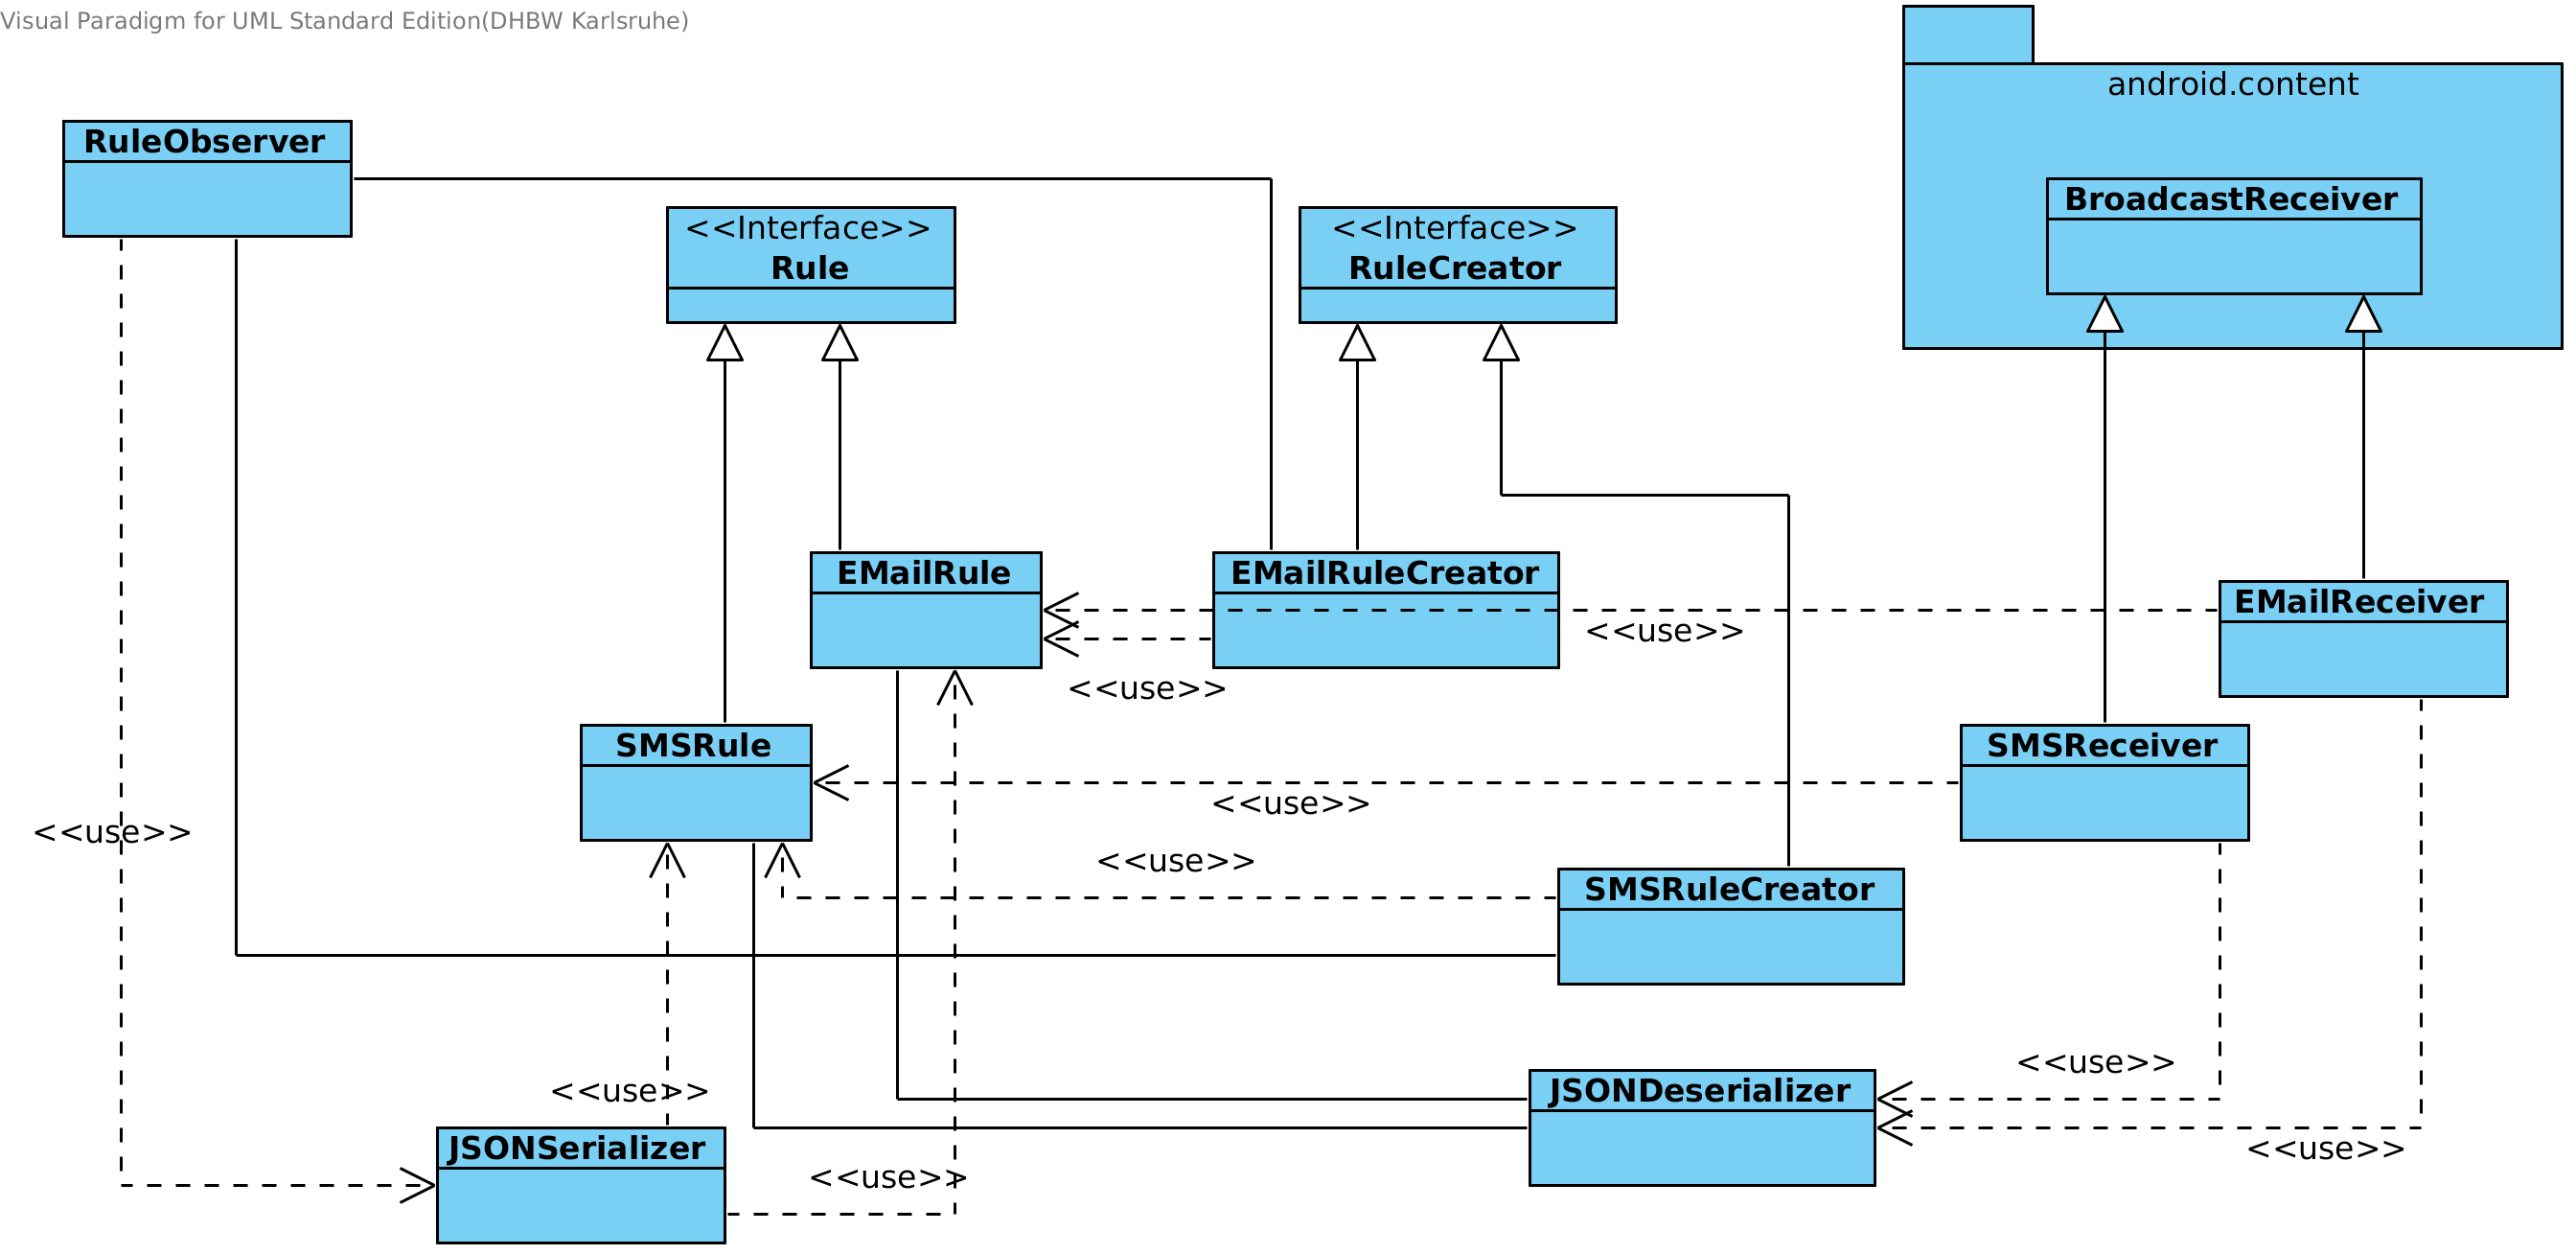
\includegraphics[width=16cm]{Bilder/AKD.png}
\caption{Analyseklassendiagramm der App}
\label{AKD}
\centering
\end{figure}